%%%%%%%%%%%%%%%%%%%%%%%%%%%%%%%%%%%%%%%%%%%%%%%%%%%%%%%%%%%%%%%%%%%%%%%%

%%% LaTeX Template for ECAI Papers 
%%% Prepared by Ulle Endriss (version 1.0 of 2023-12-10)

%%% To be used with the ECAI class file ecai.cls.
%%% You also will need a bibliography file (such as mybibfile.bib).

%%%%%%%%%%%%%%%%%%%%%%%%%%%%%%%%%%%%%%%%%%%%%%%%%%%%%%%%%%%%%%%%%%%%%%%%

%%% Start your document with the \documentclass{} command.
%%% Use the first variant for the camera-ready paper.
%%% Use the second variant for submission (for double-blind reviewing).

\documentclass{ecai} 
%\documentclass[doubleblind]{ecai} 

%%%%%%%%%%%%%%%%%%%%%%%%%%%%%%%%%%%%%%%%%%%%%%%%%%%%%%%%%%%%%%%%%%%%%%%%

%%% Load any packages you require here. 

\usepackage{latexsym}
\usepackage{amssymb}
\usepackage{amsmath}
\usepackage{amsthm}
\usepackage{booktabs}
\usepackage{enumitem}
\usepackage{graphicx}
\usepackage{color}


%%%%%%%%%%%%%%%%%%%%%%%%%%%%%%%%%%%%%%%%%%%%%%%%%%%%%%%%%%%%%%%%%%%%%%%%

%%% Define any theorem-like environments you require here.

\newtheorem{theorem}{Theorem}
\newtheorem{lemma}[theorem]{Lemma}
\newtheorem{corollary}[theorem]{Corollary}
\newtheorem{proposition}[theorem]{Proposition}
\newtheorem{fact}[theorem]{Fact}
\newtheorem{definition}{Definition}

%%%%%%%%%%%%%%%%%%%%%%%%%%%%%%%%%%%%%%%%%%%%%%%%%%%%%%%%%%%%%%%%%%%%%%%%

%%% Define any new commands you require here.

\newcommand{\BibTeX}{B\kern-.05em{\sc i\kern-.025em b}\kern-.08em\TeX}

% \def\anon{1}
\def\anon{0}

%%%%%%%%%%%%%%%%%%%%%%%%%%%%%%%%%%%%%%%%%%%%%%%%%%%%%%%%%%%%%%%%%%%%%%%%

\begin{document}

%%%%%%%%%%%%%%%%%%%%%%%%%%%%%%%%%%%%%%%%%%%%%%%%%%%%%%%%%%%%%%%%%%%%%%%%

\begin{frontmatter}

%%% Use this command to specify your submission number.
%%% In doubleblind mode, it will be printed on the first page.

\paperid{123} 

%%% Use this command to specify the title of your paper.

\title{A Time-Series Dataset of Jet Engine 

Fault Scenarios for Diagnostic Research}

%%% Use this combinations of commands to specify all authors of your 
%%% paper. Use \fnms{} and \snm{} to indicate everyone's first names 
%%% and surname. This will help the publisher with indexing the 
%%% proceedings. Please use a reasonable approximation in case your 
%%% name does not neatly split into "first names" and "surname".
%%% Specifying your ORCID digital identifier is optional. 
%%% Use the \thanks{} command to indicate one or more corresponding 
%%% authors and their email address(es). If so desired, you can specify
%%% author contributions using the \footnote{} command.

\ifnum\anon=0

\author[A]{\fnms{Christoforos}~\snm{Romesis}\orcid{0009-0001-6485-5548}\thanks{Corresponding Author. Email: chris.romesis@iit.demokritos.gr}\footnote{Equal contribution.}}
\author[A]{\fnms{Stasinos}~\snm{Konstantopoulos}\orcid{0000-0002-2586-1726}\footnotemark}
\address[A]{Institute of Informatics and Telecommunications, NCSR Demokritos}

\fi

%%% Use this environment to include an abstract of your paper.

\begin{abstract}
This paper introduces a dataset for developing and evaluating machine learning algorithms 
in gas turbine engine health monitoring. Generated using a validated Engine Performance Model 
in MATLAB, it includes time-series data simulating realistic engine conditions and faults 
across ten operating points and five health states: healthy, increased compressor blade clearance, 
compressor inlet guide vane mistuning, foreign object damage, and combined faults. Each series consists
 of 3,600 time steps, representing one hour of engine operation at 1 Hz. The dataset captures the 
 dynamic development of health conditions, including scenarios with transient and persistent faults,
  as well as complex fault interactions, offering a comprehensive resource for advancing fault diagnosis
   and prognostics in gas turbine engines. The data is available in a compressed CSV format.
\end{abstract}

\end{frontmatter}

%%%%%%%%%%%%%%%%%%%%%%%%%%%%%%%%%%%%%%%%%%%%%%%%%%%%%%%%%%%%%%%%%%%%%%%%

\section{Introduction}

Jet engines play a vital role in modern aviation, 
making the assurance of their operational safety and reliability a top priority.
The challenging high-speed, high-temperature, and high-pressure environments
in which these engines operate can compromise their integrity, 
leading to potential malfunctions or degraded performance of their components
during flight. These faults directly impact aerothermodynamic measurements 
such as pressures, temperatures, and shaft speeds, which are essential for 
condition monitoring \citep{mathioudakis_signatures_2024}. Detecting faults from time-series data in-flight 
remains a complex challenge for the research community due to limitations
in available instrumentation \citep{urban_gas_1973}, the similarity of fault effects, 
the possibility of multiple concurrent faults, and the influence of prior 
events on the development of later faults events.

In this paper, we present a dataset comprising simulated time-series 
measurements from a typical turbofan engine during flight. 
This dataset includes instances where one or more of three common 
faults—namely increased tip clearance (TIP), variable guide vane (VGV) 
mistuning, and foreign object damage (FOD)—occur. This dataset aims to 
facilitate the development and evaluation of fault detection strategies 
in aviation engine condition monitoring.

\section{Motivation and Purpose}
This dataset presents a valuable resource for the Machine Learning community
due to its embodiment of a complex engineering problem, characterized by 
several distinctive features. It comprises 2,410 time series, each with 
3,600 time steps. Within each series, one or more faults from a set of 
three are introduced, with measurements and fault labels available at every 
time step. Notably, some fault instances induce effects on the measurements 
that are nearly indistinguishable, posing significant challenges for fault 
differentiation. Additionally, certain faults exhibit long-term dependencies 
on preceding faults, serving as critical clues for accurate identification 
despite similar measurement effects. These attributes render the dataset 
highly suitable for advancing research in sequential and time-stepwise 
classification, as well as for investigating long-term dependencies within 
time-series data.


\section{Dataset Description}
The dataset comprises a time series of measurements collected from a 
low bypass ratio turbofan engine, which is representative of 
contemporary in-service civil aviation engines. The dataset was 
generated using an Engine Performance Model (EPM) that simulates the 
engine's operational behavior.

\subsection{Dataset Description}
An EPM interrelates parameters that represent engine component health and operating
conditions with measurements performed on an engine \citep{alexiou_development_2005},
and can be expressed through Equation~(\ref{eq:epm}):

\begin{eqnarray}\label{eq:epm}
\mathbf{Y} = \mathbf{g}(\mathbf{u}, \mathbf{f})
\end{eqnarray}

where $\mathbf{g}$ is a vector function representing the EPM, $\mathbf{u}$ is a vector of measured 
quantities defining the engine's operating point, $\mathbf{Y}$ is a set of measurements 
for condition monitoring, and $\mathbf{f}$ is a vector of engine component 
\textit{health parameters}. Typically, two health parameters are used for each 
component: the flow factor (SW), indicating the component's swallowing capacity,
 and the efficiency factor (SE), representing thermal efficiency. 
 The application of such parameters for assessing engine component health has 
 been discussed in \citep{mathioudakis_performance_2001}. A deviation of a health parameter from its nominal value 
 signals a fault in that component. As extensively discussed in \citep{mathioudakis_signatures_2024}   
 the ratio of deviations between two health parameters can serve as a 
 characteristic metric for faults such as fouling, increased tip clearance, 
 erosion, and foreign object damage. The severity of the 
 fault correlates with the level of this deviation. The deviation (or \textit{delta}) 
 of a health parameter $\mathbf{\Delta f}$ is defined as:

\begin{eqnarray}\label{eq:deltaf}
    \mathbf{\Delta f}\ (\%) = \frac{\mathbf{f} - \mathbf{f_o}}{\mathbf{f_o}} \cdot 100\%
\end{eqnarray}

where $\mathbf{f}$ denotes the value of the health parameter, and $\mathbf{f_o}$ its nominal value.

Using the EPM, the nominal values of the available measurement set, denoted as $\mathbf{Y_o}$, 
can be computed for a specified operating point $\mathbf{u}$. These values correspond to the nominal
health parameters, $\mathbf{f_o}$, and are derived via the following relation:

\begin{eqnarray}\label{eq:epmnom}
\mathbf{Y_o} = \mathbf{g}(\mathbf{u}, \mathbf{f_o})
\end{eqnarray}

Once a measurement vector $\mathbf{Y}$ is obtained from the engine, the percentage deviation (\textit{delta})
from its nominal value $\mathbf{Y_o}$ is defined as:

\begin{eqnarray}\label{eq:deltay}
    \mathbf{\Delta Y}\ (\%) = \frac{\mathbf{Y} - \mathbf{Y_o}}{\mathbf{Y_o}} \cdot 100\%
\end{eqnarray}



To emulate realistic measurement conditions, random noise is superimposed on the measurement 
deviations. The noise levels considered are consistent with those typical of this instrumentation, 
as documented in \citep{romesis_model-assisted_2024}.

\subsection{Dataset Generation}
The EPM used for dataset generation was developed in the MATLAB environment, following the approach 
described in \citep{alexiou_development_2005}. At each time step, the data includes a labeled vector
of measurement deltas produced by the EPM at a specified operating point (input vector $\mathbf{u}$) and a 
specific engine health condition (input vector $\mathbf{\Delta f}$).

A total of 10 operating points were considered, covering a broad range of the engine’s flight envelope.
Throughout a time series, all time steps correspond to the same operating point.

Additionally, five distinct health conditions were considered, as summarized in Table~\ref{tab:health_conditions}.
The first health condition represents the nominal, healthy operation of the engine, with no deviations in health 
parameters across any components. The second health condition (coded as TIP) models an increased clearance of the 
compressor blades. As reported in \citep{mathioudakis_signatures_2024}, this fault results in a ratio of the 
related health parameter deviations, $\Delta SW/\Delta SE$, of $0.2$; the actual deviations of $\Delta SW$ 
and $\Delta SE$ are around $-1\%$ and $-5\%$, respectively. 
The third health condition pertains to mistuning of the inlet guide vanes (VGV) of the compressor, 
analogous to the TIP fault. In these instances, deviations in the compressor’s health parameters $\Delta SW$ 
and $\Delta SE$ are typically around $+3\%$ to $-1\%$, respectively, resulting in a ratio of $-3$.
The fourth health condition involves damage caused by foreign objects (FOD) within the compressor. 
In such cases, deviations in both health parameters are generally around $-4\%$, yielding a ratio of $1$.
The fifth health condition represents the concurrent occurrence of VGV and FOD faults (denoted as VGV+FOD).
The combined effect in this scenario is additive, with deviations around $+1\%$ and $-5\%$,
respectively, leading to a ratio of $0.2$. 
In all cases, deviations within the range of 0.7 to 1.3 times the aforementioned values are considered, simulating faults of varying severity. 

Notably, the effects of TIP faults and the combined VGV+FOD faults on the compressor’s health parameters
are the same, and therefore, measurements under these conditions follow the same distribution.
Each dataset record is labeled according to the specific health condition present at that time step.

\begin{table}[h]
\caption{Considered health conditions.}
\label{tab:health_conditions}
\centering
\begin{tabular}{ccccc} 
\toprule
label &  health condition & $\Delta SE$ & $\Delta SE$ & $\Delta SW/\Delta SE$ \\
\midrule
1	& Healthy	& 0\%	& 0\%	& N/A \\
2	& TIP fault	& -1\%	& -5\%	& 0.2 \\
3	& VGV fault	& +3\%	& -1\%	& -3 \\
4	& FOD fault	& -4\%	& -4\%	& 1 \\
5	& VGV+FOD faults	& -1\%	& -5\%	& 0.2 \\
\bottomrule
\end{tabular}
\end{table}


Each time series comprises 3{,}600 time steps, representing measurements acquired from the engine
at a frequency of 1~Hz during one hour of flight at a specific operating point. During this period,
various health conditions may develop.

A time series without any fault contains measurements indicative of healthy engine operation
at all time steps (labeled $1$). In some time series, the engine operates fault-free initially
(time steps labeled $1$), but at a certain point, a TIP fault occurs and persists until the end
of the series (time steps labeled $2$). Similarly, there are series where the engine functions
without faults initially (time steps $1$), but subsequently a VGV or FOD fault occurs, 
remaining until the series concludes (time steps labeled $3$ or $4$, respectively).
In some other time series, the engine also operates fault-free initially (time steps labeled $1$),
but at a certain point, a brief period (approximately 10 time steps) occurs during which a VGV fault is
present. The engine then continues to operate without faults until a later time step, when a combined
VGV+FOD fault manifests and persists for the remainder of the time series.
This scenario exemplifies a specific fault condition characterized by a severe VGV fault leading to FOD.
The damage is attributed to the detachment of a particle from the VGV mechanism, such as a loosened bolt, which is
subsequently ingested by the engine. The failure of the VGV mechanism may be preceded by a transient VGV
fault event, serving as an early indicator of the impending failure.
This scenario was selected because both the TIP and VGV+FOD faults exert similar impacts on engine performance. The key differentiator between the TIP fault and the VGV+FOD fault is the long-term dependency of the latter on the initial, instantaneous VGV fault.


\subsection{Dataset Characteristics}

The dataset is available in compressed CSV format (csv.gz) at ... Table~\ref{tab:csv_lines} shows the first lines
 of the CSV file for illustration, displaying the header and the first three records of the dataset. 
 Table~\ref{tab:csv_records} describes the contents of each record.

\begin{table*}[t]
\caption{First lines of the csv file of the dataset.}
\label{tab:csv_lines}
\centering
\begin{tabular}{ccccccccccc} 
\toprule
TSid & Timestamp & $\Delta NH$ & $\Delta Wf$ & $\Delta Pt13$ & $\Delta Tt13$ & $\Delta Pt31$ & $\Delta Tt31$ & $\Delta Tt5$ & $\Delta Pt45$ & label \\
\midrule
1 & 1 & -0.036845 & -0.234350 & 0.076877 & -0.033296 & 0.102473 & -0.061737 & 0.063211 & -0.099636 & 1 \\
1 & 2 & -0.076961 & 0.163981 & 0.038031 & -0.002113 & -0.489823 & -0.264619 & -0.088901 & 0.002527 & 1 \\
1 & 3 & 0.086086 & -0.469731 & -0.124249 & 0.034572 & -0.049747 & 0.012047 & -0.386412 & -0.085846 & 1 \\
\bottomrule
\end{tabular}
\end{table*}


\begin{table*}[h]
\caption{Contents of the dataset’s records.}
\label{tab:csv_records}
\centering
\begin{tabular}{cccl} 
\toprule
Header &  Type & Values & Description \\
\midrule
DNH & float64 & $[-1.617629, 1.391620]$ & percentage deviation of measurement: NH (high-pressure shaft speed) \\
DWf & float64 & $[-1.502119, 9.226637]$ & percentage deviation of measurement: Wf (fuel mass flow) \\
DPt13 & float64 & $[-0.590554, 4.295775]$ & percentage deviation of measurement: Pt13 (fan inlet total pressure) \\
DTt13 & float64 & $[-0.484075, 1.393903]$ & percentage deviation of measurement: Tt13 (fan inlet total temperature) \\
DPt31 & float64 & $[-1.006958, 2.094033]$ & percentage deviation of measurement: Pt31 (compressor inlet total pressure) \\
DTt31 & float64 & $[-0.456074, 3.547797]$ & percentage deviation of measurement: Tt31 (compressor inlet total temperature) \\
DTt5 & float64 & $[-0.832501, 7.432680]$ & percentage deviation of measurement: Tt5 (turbine outlet total temperature) \\
DPt45 & float64 & $[-0.749605, 2.305785]$ & percentage deviation of measurement: Pt45 (interturbine total pressure) \\
label & integer & $[1, 5]$ & health condition label \\

\bottomrule
\end{tabular}
\end{table*}

\section{Example Application}
The dataset is currently employed to evaluate the classification capabilities of various sequential machine learning methods applied to time-series data characterized by long-term dependencies. Although this is an ongoing study, preliminary results suggest that the dataset presents a challenging use case that tests the limits of current state-of-the-art techniques. Figure~\ref{fig:results} illustrates an example of these results, where four classification methods trained on the dataset are tested on a time-series segment containing a VGV+FOD fault. The methods include an RNN, a GRU, and an LSTM, along with an MLP trained for point-to-point classification for comparison. At each time step, the actual health condition is depicted in blue, while the estimated condition is shown in red. The results indicate that all methods fail to detect the VGV+FOD fault, which occurs around time step 3200, although a sudden event—a VGV fault at approximately time step 740 that serves as a precursor to the VGV+FOD fault —is detected by all methods. Thus far, sequential methods have shown limited ability to leverage information from prior time steps, performing similarly to the point-wise MLP.  


\begin{figure}[h]
  \centering
  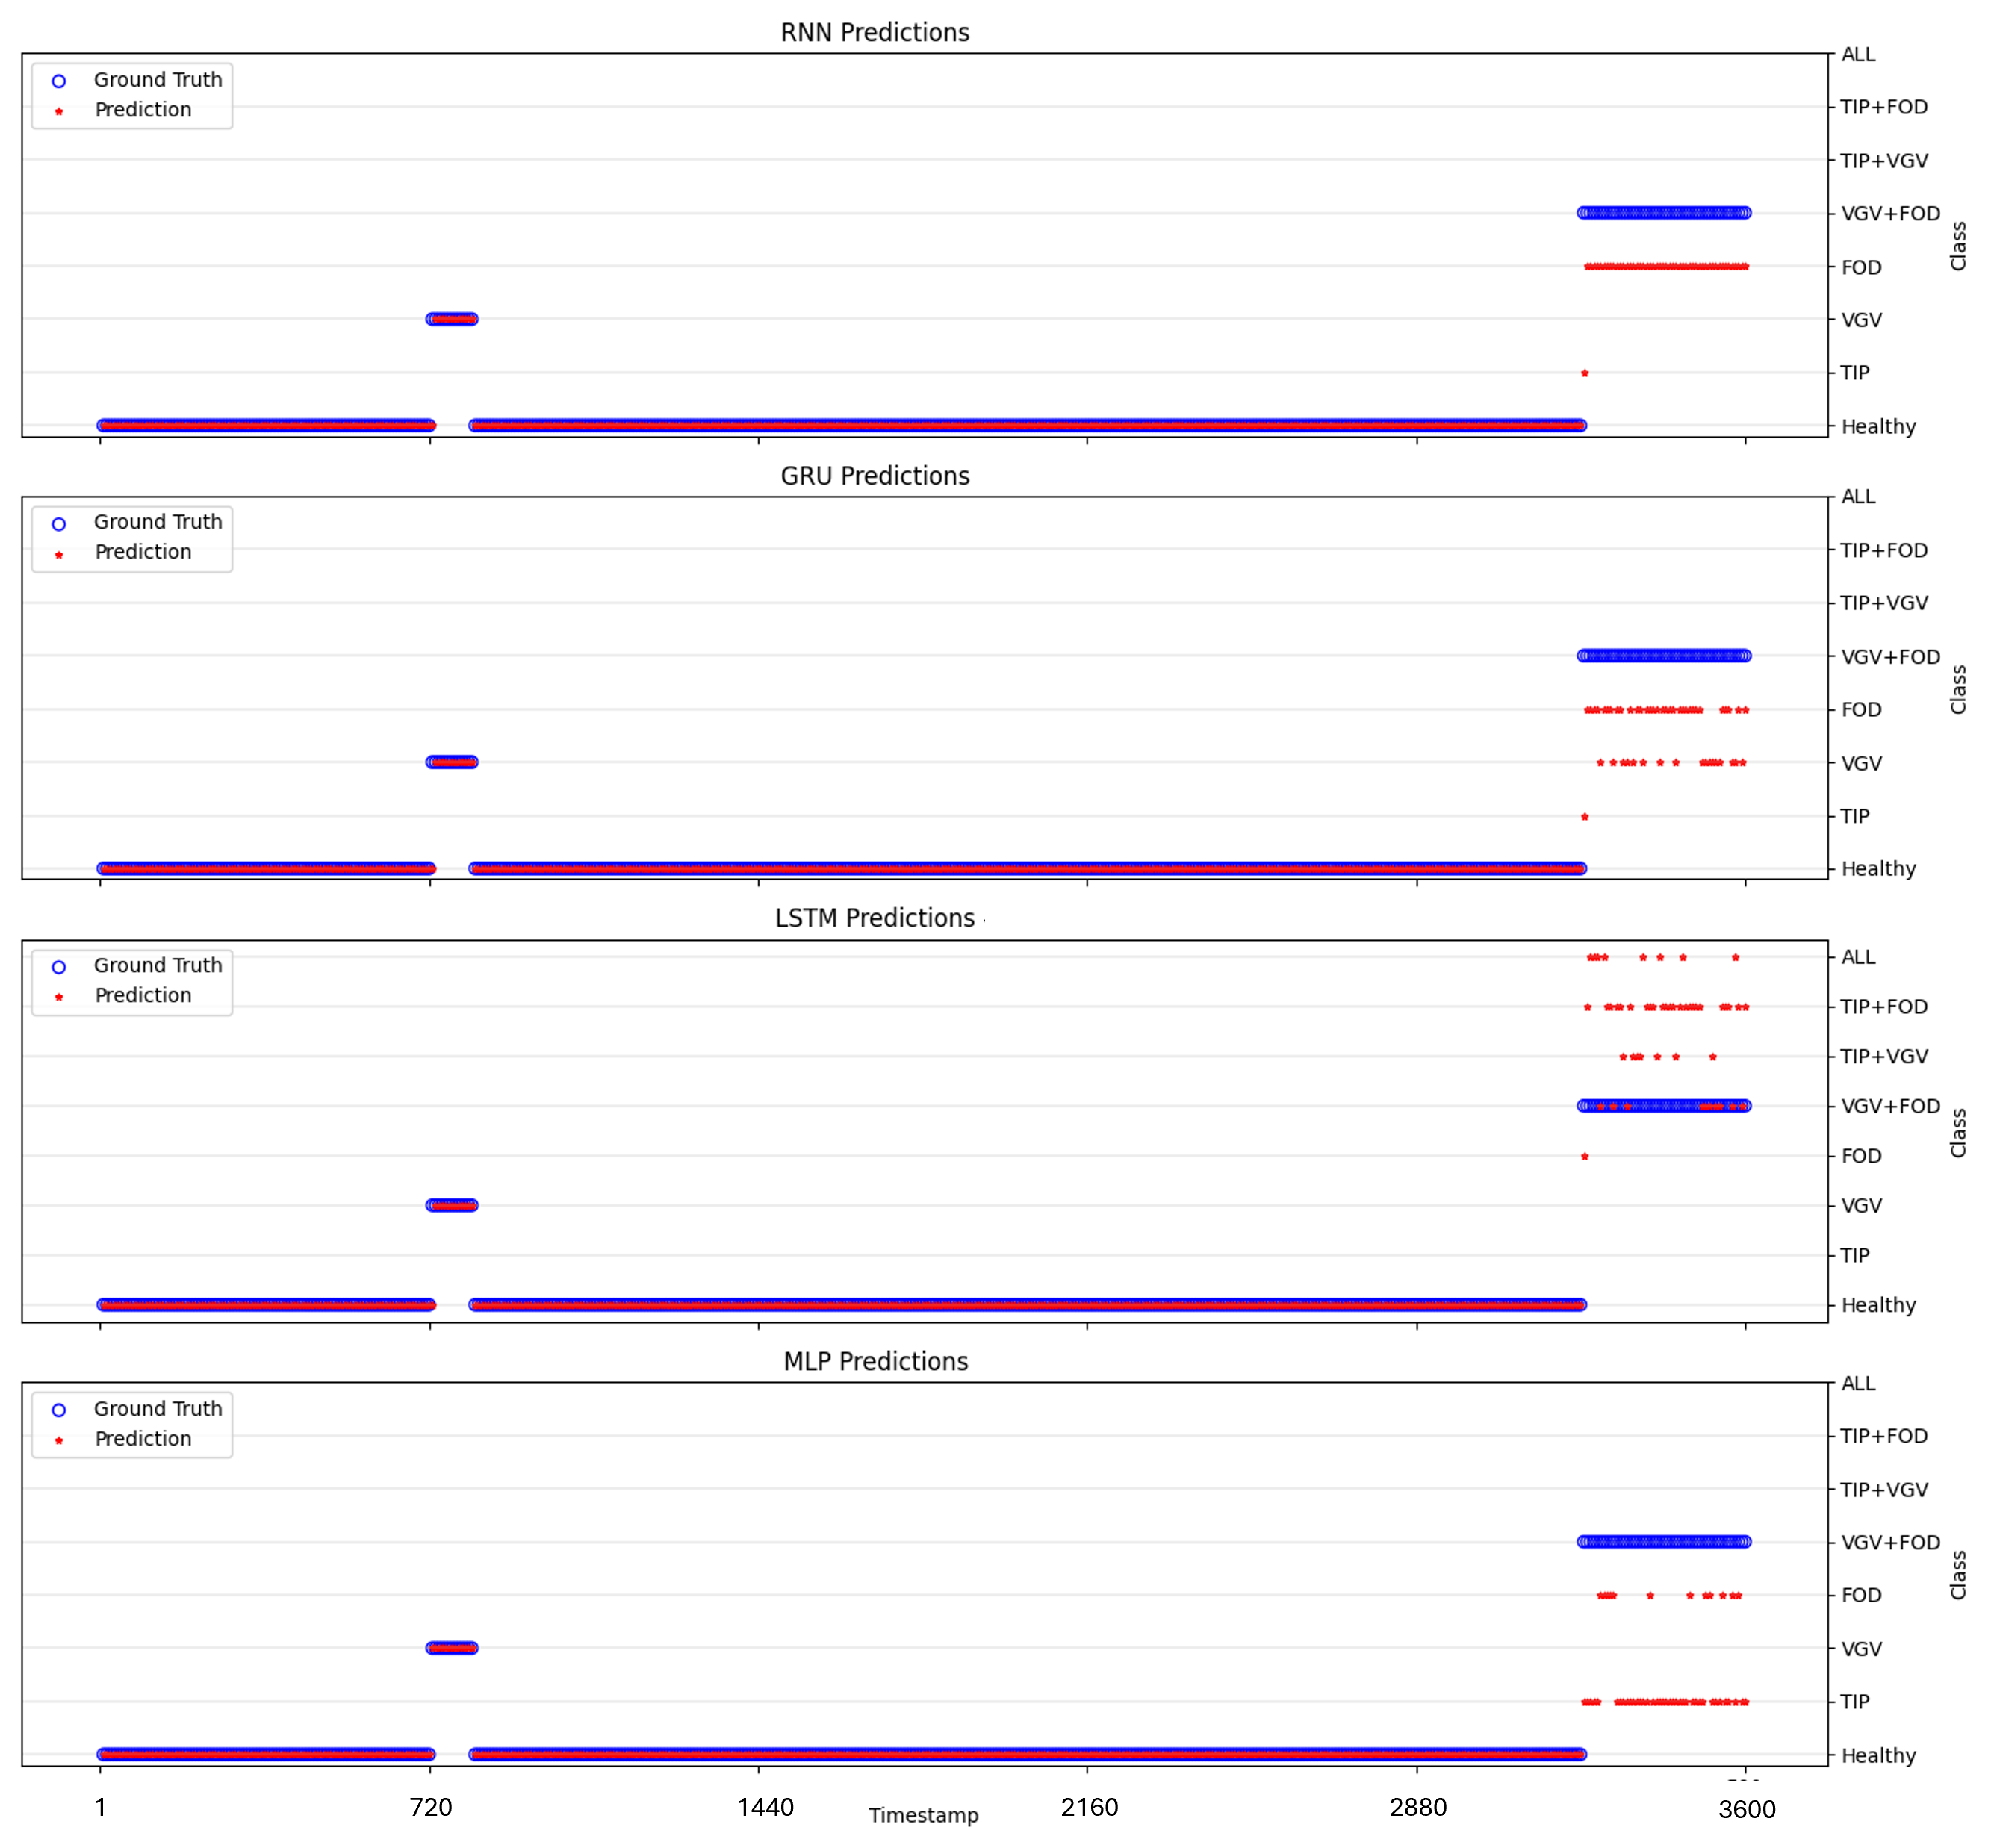
\includegraphics[width=8.5cm]{comparison_eval_tsid_8_mod}
  \caption{Development of health conditions during a time-series of the dataset.}
  \label{fig:results}
\end{figure}


\section{Conclusions}

A novel dataset for gas turbine engine health monitoring has been generated using a validated Engine Performance Model within a MATLAB environment. This dataset encompasses a range of operating conditions and fault scenarios, providing a comprehensive resource 
for the development and evaluation of machine learning algorithms. By including various 
health conditions, such as increased compressor blade clearance, compressor inlet guide 
vane mistuning, foreign object damage, and concurrent faults, the dataset enables the 
study of complex fault interactions and the development of robust diagnostic tools. 
The time-series data, with measurements acquired at a 1 Hz frequency, captures the 
dynamic development of health conditions, including transient and persistent faults. 
Its features make it especially useful for research in sequential and time-step 
classification, as well as for analyzing long-term dependencies in data. 
The dataset's structure and characteristics are detailed to ensure its accessibility 
and usability for researchers and practitioners in the field.



%%%%%%%%%%%%%%%%%%%%%%%%%%%%%%%%%%%%%%%%%%%%%%%%%%%%%%%%%%%%%%%%%%%%%%%%

% \section{References}

% Include full bibliographic information for everything you cite, 
% be it a book \citep{pearl2009causality}, a journal article 
% \citep{grosz1996collaborative,rumelhart1986learning,turing1950computing}, 
% a conference paper \citep{kautz1992planning}, or a preprint 
% \citep{perelman2002entropy}. The citations in the previous sentence are 
% known as \emph{parenthetical} citations, while this reference to the 
% work of \citet{turing1950computing} is an \emph{in-text} citation.
% The use of \BibTeX\ is highly recommended. 

%%%%%%%%%%%%%%%%%%%%%%%%%%%%%%%%%%%%%%%%%%%%%%%%%%%%%%%%%%%%%%%%%%%%%%%%

%%% Use this environment to include acknowledgements (optional).
%%% This will be omitted in doubleblind mode.

% \begin{ack}
% By using the \texttt{ack} environment to insert your (optional) 
% acknowledgements, you can ensure that the text is suppressed whenever 
% you use the \texttt{doubleblind} option. In the final version, 
% acknowledgements may be included on the extra page intended for references.
% \end{ack}

%%%%%%%%%%%%%%%%%%%%%%%%%%%%%%%%%%%%%%%%%%%%%%%%%%%%%%%%%%%%%%%%%%%%%%%%

%%% Use this command to include your bibliography file.

\bibliography{mybibfile} % Unsorted references – uses citation order


\end{document}
%%%%%%%%%%%%%%%%%%%%%%%%%%%%%%%%%%%%%%%%%%%%%%%%%%%%%%%%%%%%%%%%%%%%%%
